% Use class option [extendedabs] to prepare the 1-page extended abstract.
\documentclass[extendedabs]{bmvc2k}
\usepackage[colorlinks = true,
            linkcolor = blue,
            urlcolor  = blue,
            citecolor = blue,
            anchorcolor = blue]{hyperref}
\usepackage{kotex}
% for the fancy \koTeX logo
\usepackage{kotex-logo}
\usepackage{mathtools}  % brings in amsmath, also some improvements
\usepackage{amssymb} % brings in amsfonts, incl \square
% Document starts here
\usepackage{graphicx}
\begin{document}


\title{Vision Transformer final-report}
\addauthor{
Taehun Kim$^{1}$
}{}{1}

\addinstitution{
$^1$ Department of Computer Science and Engineering, Pusan National University.  
}
 

\maketitle
\noindent

\section{Introduction}
The Vision Transformer\cite{vit} is a model that directly applies the Transformer\cite{transformer} architecture to image. this model achieves excellent results when pre-trained at large scale and transferred to tasks with fewer datapoints.

In this report, We test the Vision Transformer, visualize its attention matrix. We use pre-trained Vision Transformer from TIMM(pytorch image model)\cite{rw2019timm} with $16\times16$ patch size and $224\times224$ input image size. The Vision Transformer implementation is from \cite{rw2019timmvit}.
\section{Test data}
We use the Santorini image from \cite{santorini}. the image is resized to $224\times224$, and normalized with mean of 0.5 and a standard deviation of 0.5.
\section{Vision Transformer}
In this section, we examine the details of the Vision Transformer by implementing a small part of the model. The architecure of the Vision Transformer is shown in Figure \ref{vitarch} and Figure \ref{encoderarch}.
\subsection{Patch Embedding}
We use $224\times224$ image, and divide it into patches of $16\times16$ size. This creates a grid size of $14\times14$, resulting in 196 patches. We use convolutional layers to embed each patch into a $1\times768$. 

this convolutional layer has 3 input channels, 768 output channels, $16\times16$ kernel size, and $16\times16$ stride. After each patch passes through the convolutional layer, the embedded vectors are flattened from $14\times14\times768$ to $196\times768$.
\subsection{Position Embedding}
In this report, We use pre-trained position embedding. To visualize the position embedding, We calculate the cosine similarity between one patch and all other patches and reshape the similarity vector back to the original patch grid shape. The visualization is shown in Figure \ref{posembedsimilar}. 

In the visualization, brighter areas in each patch indicate a higher similarity between the position embeddings corresponding to the rows and columns of that patch. These embeddings are more similar when aligned horizontally than vertically.
\subsection{Transformer Input}
We generate inputs for transformer using pre-trained patch and position embedding. After concatenating class token to the patch embedding, The position embedding is added to patch embedding, which finally produce input for transformer. The class token is already concatenated to position embedding. The input shape is $197\times768$.

The formula is
$$
\textbf{z}_0 = [\textbf{x}_{class};\textbf{x}_1^p\textbf{E};\textbf{x}_2^p\textbf{E};\cdots;\textbf{x}_N^p\textbf{E}]+\textbf{E}_{pos},
\textbf{E}\in \mathbb{R}^{(P^2\cdot C)\times D}, \textbf{E}_{pos} \in \mathbb{R}^{(N+1)\times D} 
$$
, which P is patch size, C is input channel, D is output channel(embedding dimension), and N is number of patches. In this lab, P is 16, C is 3, D is 768, N is 196.

\subsection{Transformer Encoder}
The transformer input is fed to L(=12) series Transformer Encoders for multihead self-attention. The embedded vector input is expanded to $197\times(3\times768)$ by a fully connected layer. this vector is divided into 3 $197\times768$ vectors: \textbf{q},\textbf{k}, and \textbf{v}. 

After that, Each vectors is divided into 12 $197\times64$ vectors, one for each attention head.
The output from the attention heads is concatenated and reshaped to match the encoder's input shape. After applying the attention heads, the result passes through layer normalization and two fully connected  layers to produce the encoder's output. We use pre-trained transformer encoder in this lab.

The formula for attention head is
$$
A = \textbf{softmax}(\textbf{q}\textbf{k}^T / \sqrt{D_h})
$$
$$
SA(\textbf{z}) = A\textbf{v}
$$
$$
MSA(\textbf{z}) = [SA_1(z);SA_2(z);\cdots;SA_k(z)]U_{msa}, U_{msa}\in \mathbb{R}^{k\cdot D_h \times D}
$$
, which A is the attention matrix, k is number of self-attention operation, $D_h$ is dimension of each head(typically set to D/k), and $U_{msa}$ is projection matrix. In this lab, k is 12, $D_h$ is 64. 

The shape of $\textbf{q}$ is $197\times64$, and $\textbf{k}^T$ is $64\times197$. Therefore, the shape of attention score is $197\times197$. The softmax layer makes the sum of each row to 1.
\subsubsection{Visualizing attention matrix}
In this section, We visualize attention matrix of the Santorini image. Typically, Layer normalization is applied after self-attention(i.e., after multiplication of Attention matrix and $\textbf{v})$. However, We applied layer normalization to a Attention matrix for visualizing. Therefore, The attention matrix for visualizing is:
$$
A_{visual} = \textbf{layernorm}(\textbf{softmax}(\textbf{q}\textbf{k}^T / \sqrt{D_h}))
$$

The visualization of the attention matrix of 4th head is shown in Figure \ref{fig:attentionvis1}. Additionally, the visualization of the 100th row of attention matrix of 0-7th heads is shown in Figure \ref{fig:attentionvis2}. Each 196 columns(except class token) is reshaped to $14\times14$. In the attention matrix visualization, the bright regions indicate that the vision transformer pays more attention to those parts of the image.

\subsection{MLP for classification}
Output of the transformer encoder is fed to MLP head, which is fully connected layer that maps 768 features to 1000 classifications. MLP head layer is also pre-trained. We only check the first rows of the output of the MLP head, corresponding to the class token index. The classification result is shown in Figure \ref{fig:classificationres}.

\section{conclusion}
We implemented the part of Vision Transformer\cite{vit}, and examine and tested the pre-trained Vision Transformer model. We visualize the position embedding and attention matrix. Additionally, we comfirmed that the pre-trained ViT could classify the Santorini image correctly. As a result, We verified that the Transformer\cite{transformer} can be directly applied to a image, attend to crucial parts of the image, and classify the image correctly.

\begin{figure}[t]
\centering
	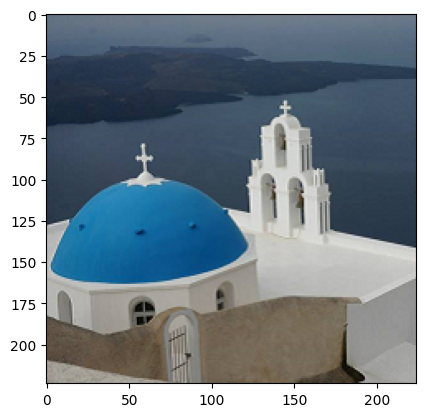
\includegraphics[width=0.5\linewidth]{images/fig1.png}
	\caption{
		Santorini image for testing ViT. The pre-trained ViT model classifies this image as 'church' and 'church building.'}
	\vspace{-2mm}
\end{figure}

\begin{figure}[t]
\centering
	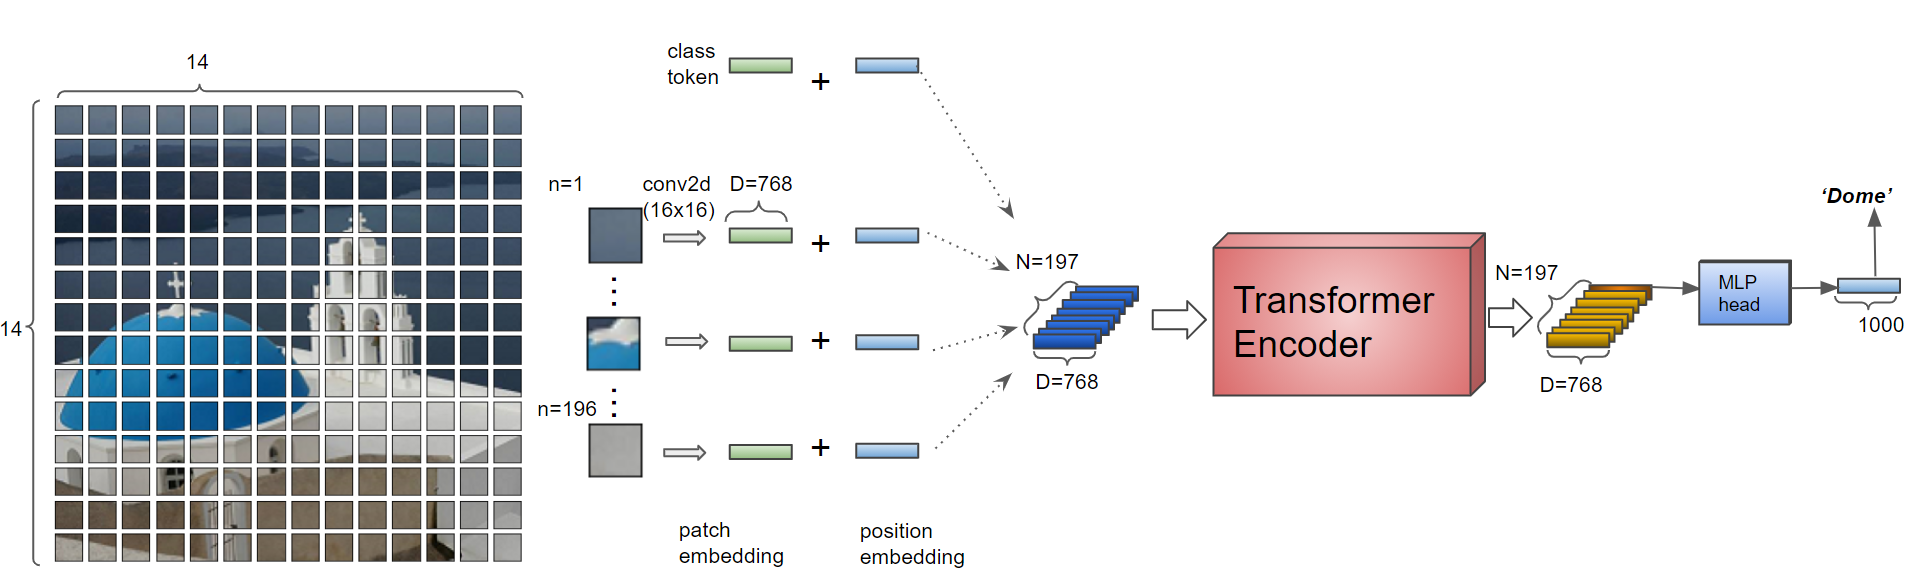
\includegraphics[width=\linewidth]{images/fig2.png}
	\caption{
		The architecture of Vision Transformer. This model divides the image into $16x\times16$ patches(196 patches from $224\times224$ image), embedding each patch to $1\times768$ by $16\times16\times768$ convolutional layers. After that, this embedded patches are added to each position embedding. This added embedded vector is fed into the Transformer Encoder. The output of the encoder is passed to an MLP head, which finally produces the classification result. }
	\vspace{-2mm}
    \label{vitarch}
\end{figure}

\begin{figure}[t]
\centering
	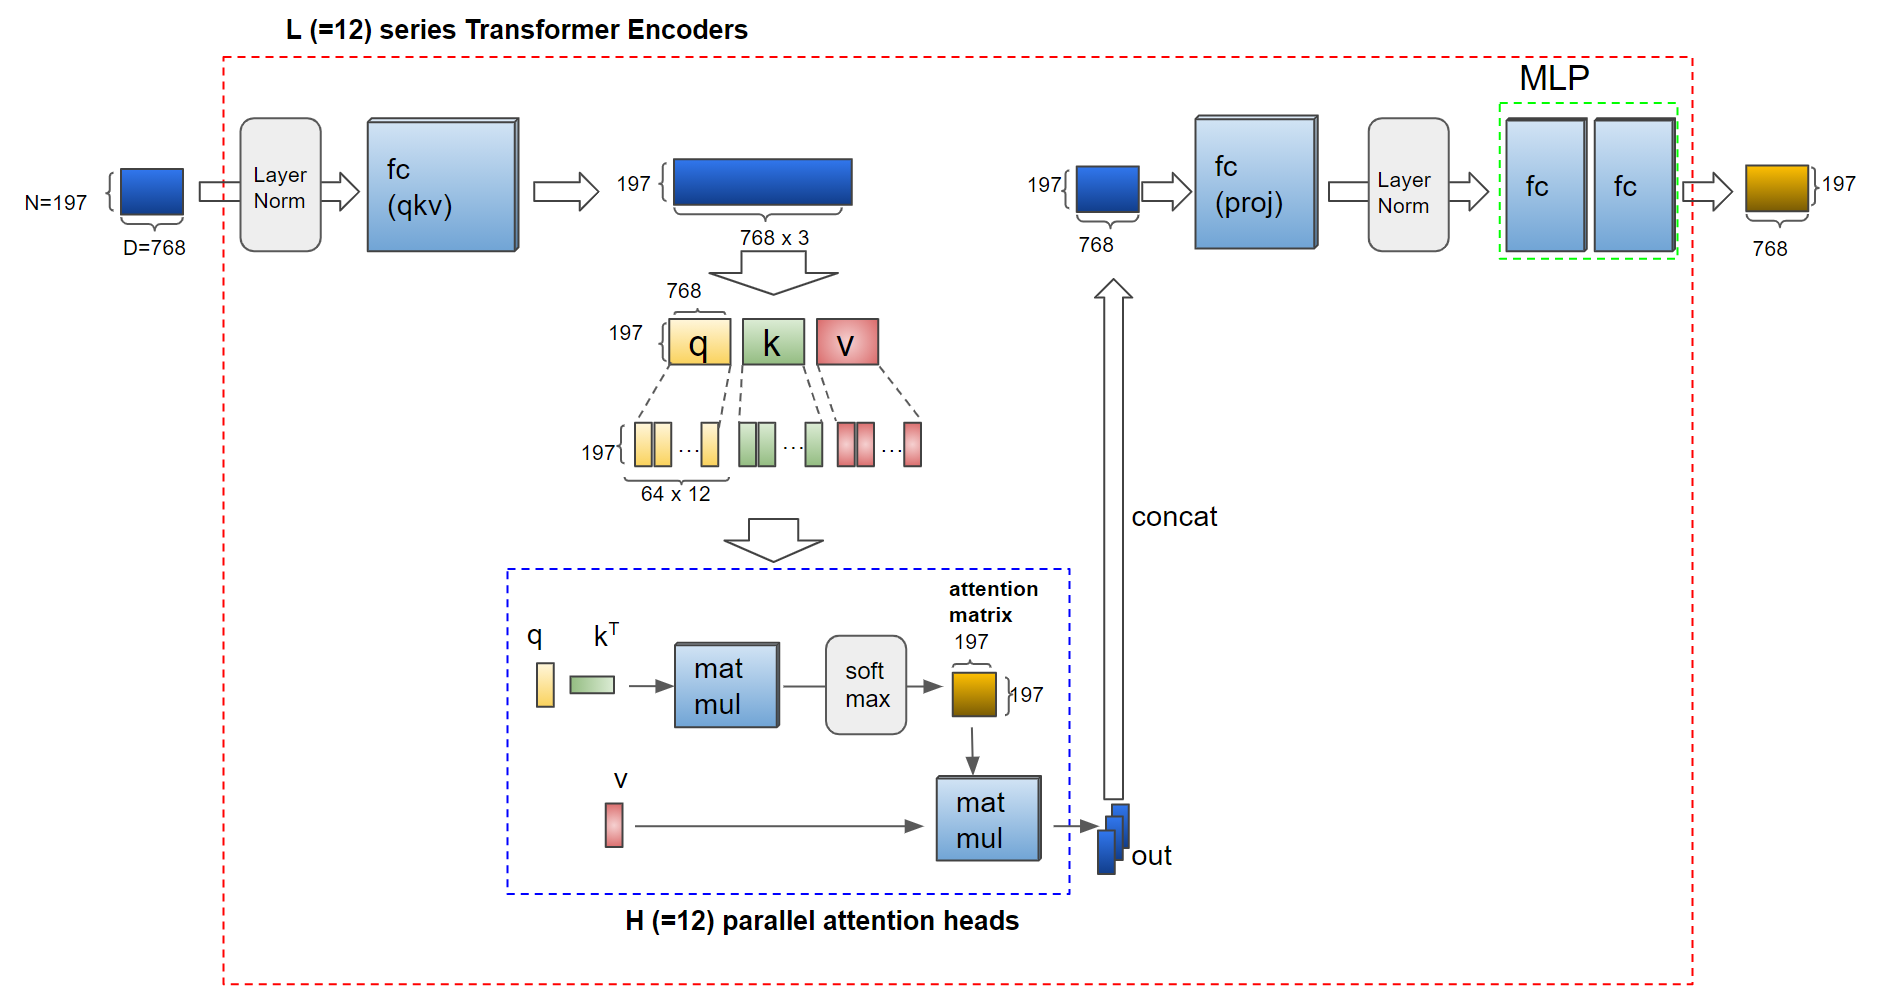
\includegraphics[width=\linewidth]{images/fig3.png}
	\caption{
		The architecture of Transformer Encoder. This encoder takes $197\times768$ embedded vector as input. After applying the layer normalization to the input, this input is fed to a fully connected layer, which produce $197\times(3\times768)$ vector. this vector is divided into 3 $197\times768$ vectors, which are the q,k,v vectors. For multi-head attention, these vector divided into 12 $197\times64$ each, and each divided vector is changed to attention matrix through matrix multiplication and softmax. The output from the attention heads is concatenated and reshaped to match the same shape as the encoder's input. After applying the attention heads, the result passes through layer normalization and two fully connected (FC) layers to produce the encoder's output.}
	\vspace{-2mm}
    \label{encoderarch}
\end{figure}


\begin{figure}[t]
\centering
\centering
	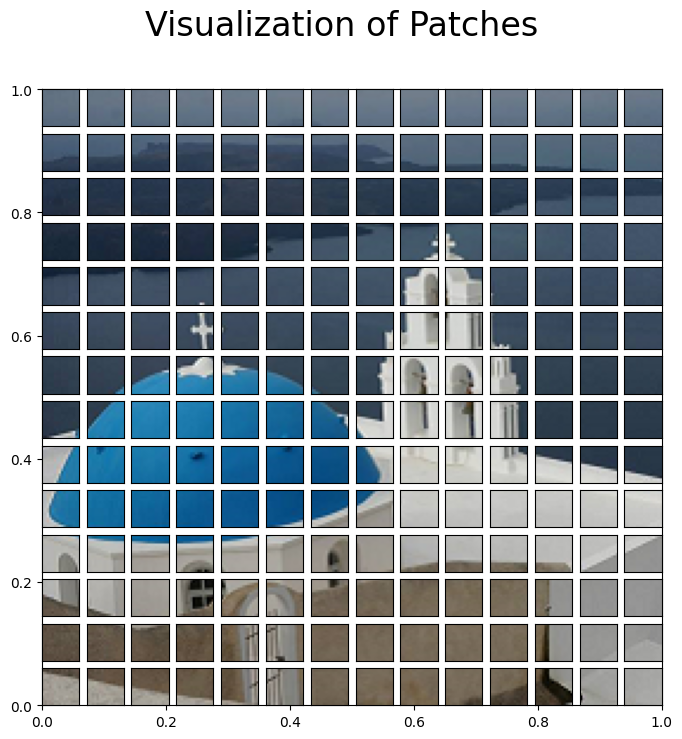
\includegraphics[width=0.5\linewidth]{images/fig4.png}
	\caption{
		Visualization of patches.}
	\vspace{-2mm}
    
\end{figure}

\begin{figure}[t]
\centering
	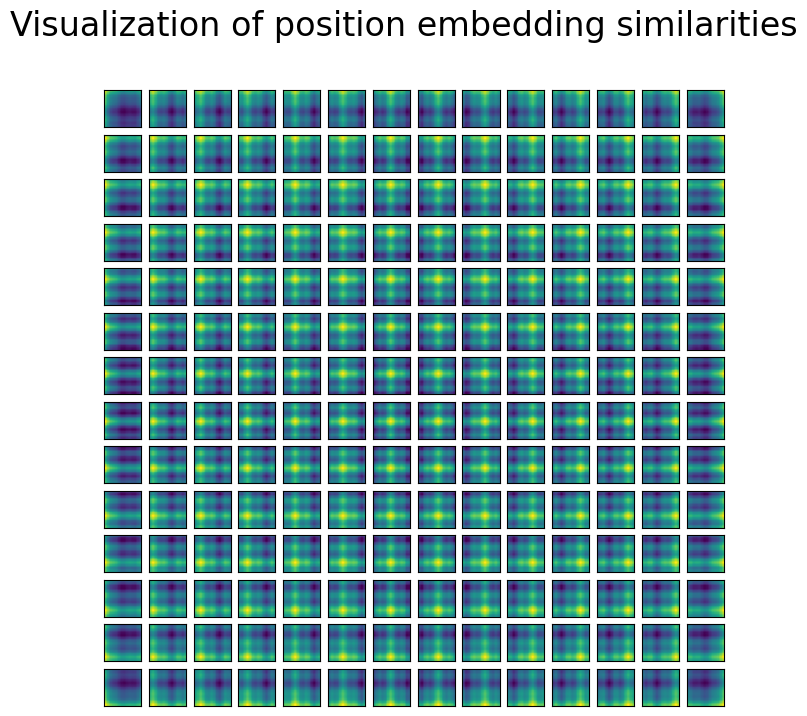
\includegraphics[width=\linewidth]{images/fig5.png}
	\caption{
		Visualization of position embedding similarities.}
	\vspace{-2mm}
        \label{posembedsimilar}
\end{figure}

\begin{figure}[t]
\centering
	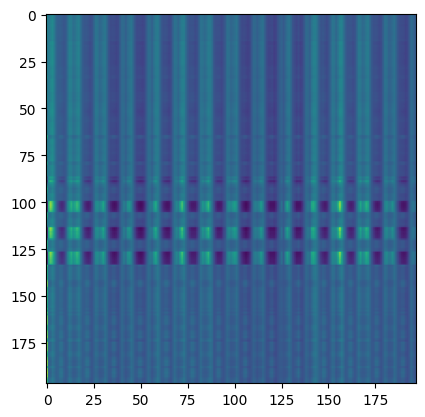
\includegraphics[width=0.7\linewidth]{images/fig6.png}
	\caption{
		Visualization of attention matrix of 4th head. The input image is the Santorini image. the size of attention matrix is $197\times197$}
	\vspace{-2mm}
        \label{fig:attentionvis1}
\end{figure}


\begin{figure}[thb] \centering
    
    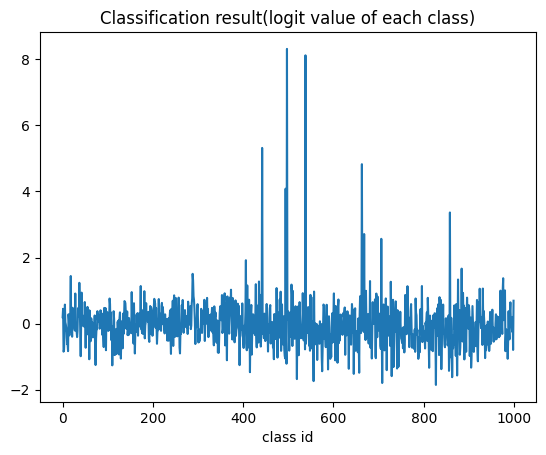
\includegraphics[width=0.5\textwidth]{images/fig8.png}
    
    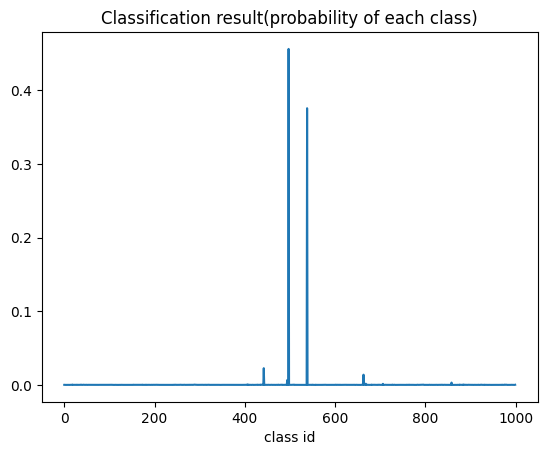
\includegraphics[width=0.5\textwidth]{images/fig9.png} 
    
    \caption{The classification result of the Santorini image using Vision Transformer. top is the logit values by class, and bottom is the probability by class. The highest class index is 497, which is corresponded to Church(and Church-building)} \label{fig:classificationres}
\end{figure}

\begin{figure}[t]
\centering
\rotatebox{90}{ % 90도 회전
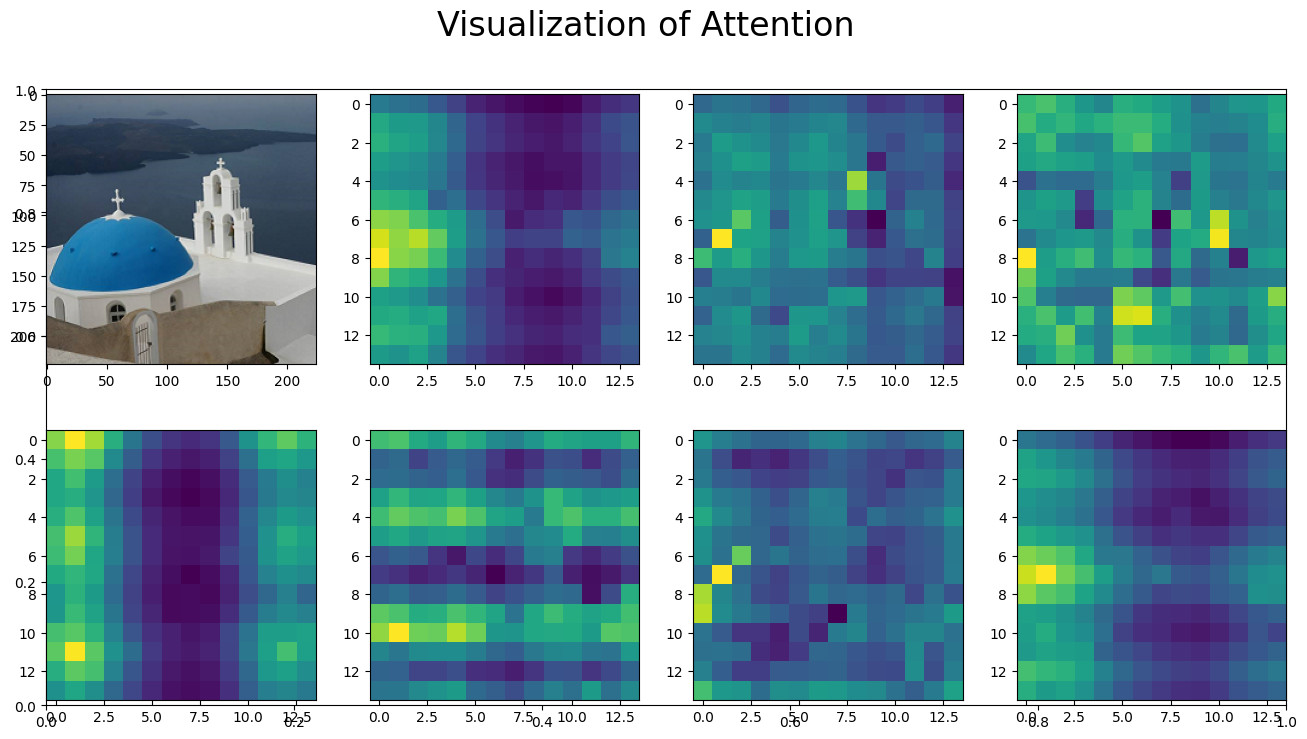
\includegraphics[width=\textwidth]{images/fig7.png}
}
	
	\caption{
		Visualization of 100th row of attention matrix of 0-7 heads. The bright regions indicate that the vision transformer pays more attention to those parts of the image.}
	\vspace{-2mm}
        \label{fig:attentionvis2}
\end{figure}

\newpage
\bibliography{egbib}

\end{document}
